\documentclass[conference]{IEEEtran}
\IEEEoverridecommandlockouts
% The preceding line is only needed to identify funding in the first footnote. If that is unneeded, please comment it out.
%Template version as of 6/27/2024

\usepackage{cite}
\usepackage{amsmath,amssymb,amsfonts}
\usepackage{algorithmic}
\usepackage{graphicx}
\usepackage{textcomp}
\usepackage{xcolor}
\usepackage{bm}

\def\BibTeX{{\rm B\kern-.05em{\sc i\kern-.025em b}\kern-.08em
    T\kern-.1667em\lower.7ex\hbox{E}\kern-.125emX}}
\begin{document}

\title{Target Speaker Extraction using Discrete Representations from 
Self-Supervised Models and Language Models
\thanks{Identify applicable funding agency here. If none, delete this.}
}

\author{\IEEEauthorblockN{1\textsuperscript{st} Beilong Tang}
\IEEEauthorblockA{\textit{Duke Kunshan University} \\
% \textit{name of organization (of Aff.)}\\
Kunshan, China \\
bt132@duke.edu}
\and
\IEEEauthorblockN{2\textsuperscript{nd} Given Name Surname}
\IEEEauthorblockA{\textit{dept. name of organization (of Aff.)} \\
\textit{name of organization (of Aff.)}\\
City, Country \\
email address or ORCID}
\and
\IEEEauthorblockN{3\textsuperscript{rd} Given Name Surname}
\IEEEauthorblockA{\textit{dept. name of organization (of Aff.)} \\
\textit{name of organization (of Aff.)}\\
City, Country \\
email address or ORCID}
% \and
% \IEEEauthorblockN{4\textsuperscript{th} Given Name Surname}
% \IEEEauthorblockA{\textit{dept. name of organization (of Aff.)} \\
% \textit{name of organization (of Aff.)}\\
% City, Country \\
% email address or ORCID}
% \and
% \IEEEauthorblockN{5\textsuperscript{th} Given Name Surname}
% \IEEEauthorblockA{\textit{dept. name of organization (of Aff.)} \\
% \textit{name of organization (of Aff.)}\\
% City, Country \\
% email address or ORCID}
% \and
% \IEEEauthorblockN{6\textsuperscript{th} Given Name Surname}
% \IEEEauthorblockA{\textit{dept. name of organization (of Aff.)} \\
% \textit{name of organization (of Aff.)}\\
% City, Country \\
% email address or ORCID}
}

\maketitle

\begin{abstract}
This document is a model and instructions for \LaTeX.
This and the IEEEtran.cls file define the components of your paper [title, text, heads, etc.]. *CRITICAL: Do Not Use Symbols, Special Characters, Footnotes, 
or Math in Paper Title or Abstract. 
\end{abstract}

\begin{IEEEkeywords}
target speaker extraction, speech separation, language models, audio discretization
\end{IEEEkeywords}

\section{Introduction}
Speech separation, the so-called cocktail party problem \cite{cocktail}, focuses on separating each individual speaker's source from a mixture with multiple speakers. This task is easy for humans but not for computers. 
In real life, speech signals are usually companied with background noise or other speakers' speeches. 
These corrupted signals may not be optimal for tasks like speaker verification \cite{rao2019targetspeakerextractionoverlapped,9414017}, and speech recognition \cite{molkov2017SpeakerAwareNN, 8462661}, emphasizing the importance of having good and robust 
speech separation models.

Unlike blind speech separation, which focuses on separating each utterance from a mixture 
of known speakers, target speaker extraction aims at only extracting the 
target speaker's voice given another auxiliary information of the target speaker. Due to the 
development of Deep Neural Network (DNN), many models nowadays are discriminative models. They 
utilize a masking strategy to minimize the distance between the clean speech and estimated 
speech directly \cite{luo2019conv,spex_plus,sepformer,sef_net}. However, these discriminative 
models may not generalize well to unseen data and might even introduce unwanted distortions \cite{distortion}. To solve these issues, researchers have proposed generative models. This method aims to learn the underlying distribution of the target speaker's voice and use this knowledge to generate the clean speech of the target speaker from a mixture of voices rather 
than directly mapping from mixed speech to clean speech. Some generative models, like diffusion
models \cite{target_diff} and variational autoencoders (VAE) \cite{vae} have been studied. It has been demonstrated that generative models can achieve results comparable to those of discriminative models \cite{target_diff,tokensplit}.

Discretization of audio has been studied due to the advancement of language models (LM). 
This approach translates the audio into discrete tokens simulating text vocabularies and uses LMs to 
model them. This approach simplifies audio generation tasks by transforming the complex 
regression problems into classification problems \cite{dasb}. There are currently two approaches for
audio discretization, the first one uses neural audio codecs \cite{dac}. This approach 
typically captures the acoustic features of the audio \cite{speech_tokenizer}. The second approach 
utilizes  self-supervised Learning (SSL) models like HuBERT \cite{hubert} and WavLM \cite{wavlm}.
SSL models have demonstrated 
excellent performances on many downstream tasks \cite{superb}. These SSL models extract  
continuous representations containing rich semantic and timbre information from a given speech. 
As demonstrated in \cite{dasb}, SSL models perform better than audio codec in tasks like speech 
enhancement and speech separation. Therefore, in this 
paper, we mainly explore the discretization of SSL models.  

Discretization methods have been studied for speech 
enhancement \cite{selm} and blind speech separation \cite{dasb,tokensplit}, 
however, this approach has 
been rarely studied for target speaker extraction. In this paper, we present a novel way to do 
target speaker extraction using discrete tokens and LMs (TSELM). Inspired by the blind speech separation 
networks proposed in DASB \cite{dasb}, our model has three stages: encoding, modeling and decoding.
For the encoding stage, reference speech and mixed speech are tokenized using WavLM and 
Kmeans as tokenizer. Unlike SELM \cite{selm}, which uses the 6th layer of WavLM as input to the Kmeans layer, 
we follow the recipes in \cite{dasb} and uses the output from hidden 
layers 1, 3, 7, 12, 18, 23 of WavLM as input to the Kmeans layer. 6 Kmeans models
are trained and applied on each layer output respectively. 
Our results indicate that using multiple layers as 
input is better 
than using only the 6th layer. The reference speech is fed to the encoder directly. 
However, for the mixed speech, instead of directly passing it to the WavLM model, we first concatenated the reference speech on both sides 
of it before passing. After tokenization, we use only the tokens 
corresponding to the mixed speech. For the modeling stage, we utilized an attention 
embedding mechanism to add each embeddings of all layers together. We used a Cross 
Attention mechanism similar in \cite{sef_net} to inject the speaker information. 
An encoder-only LM, following by a linear classifier, is applied after the cross attention module
to output the reconstructed tokens. 
For the decoding stage, we used the pretrained unit HiFi-GAN 
in \cite{unit_hifi} to reconstruct the 
discrete tokens back to audio. Unlike SELM \cite{selm}, where a conformer 
detokenizer is trained 
to reconstruct the WavLM embeddings using Kmeans center embeddings before HiFi-GAN, \cite{unit_hifi} has proposed a scalable HiFi-GAN using dropout mechanism to directly 
reconstruct audio from multiple layers of tokens without a conformer detokenizer. It 
has also eliminated the trouble of training a HiFi-GAN for each layer. The encoder and 
decoder is freezed during the training. The model overview is in Fig.\ref{model}. 
Through extensive studies, we have demonstrated this method has achieved comparable results in terms 
of speech quality and intelligibility. To the best of our knowledge, we are the first to explore 
using discrete tokens to conduct target speaker extraction.




\begin{figure*}[t]
\centering
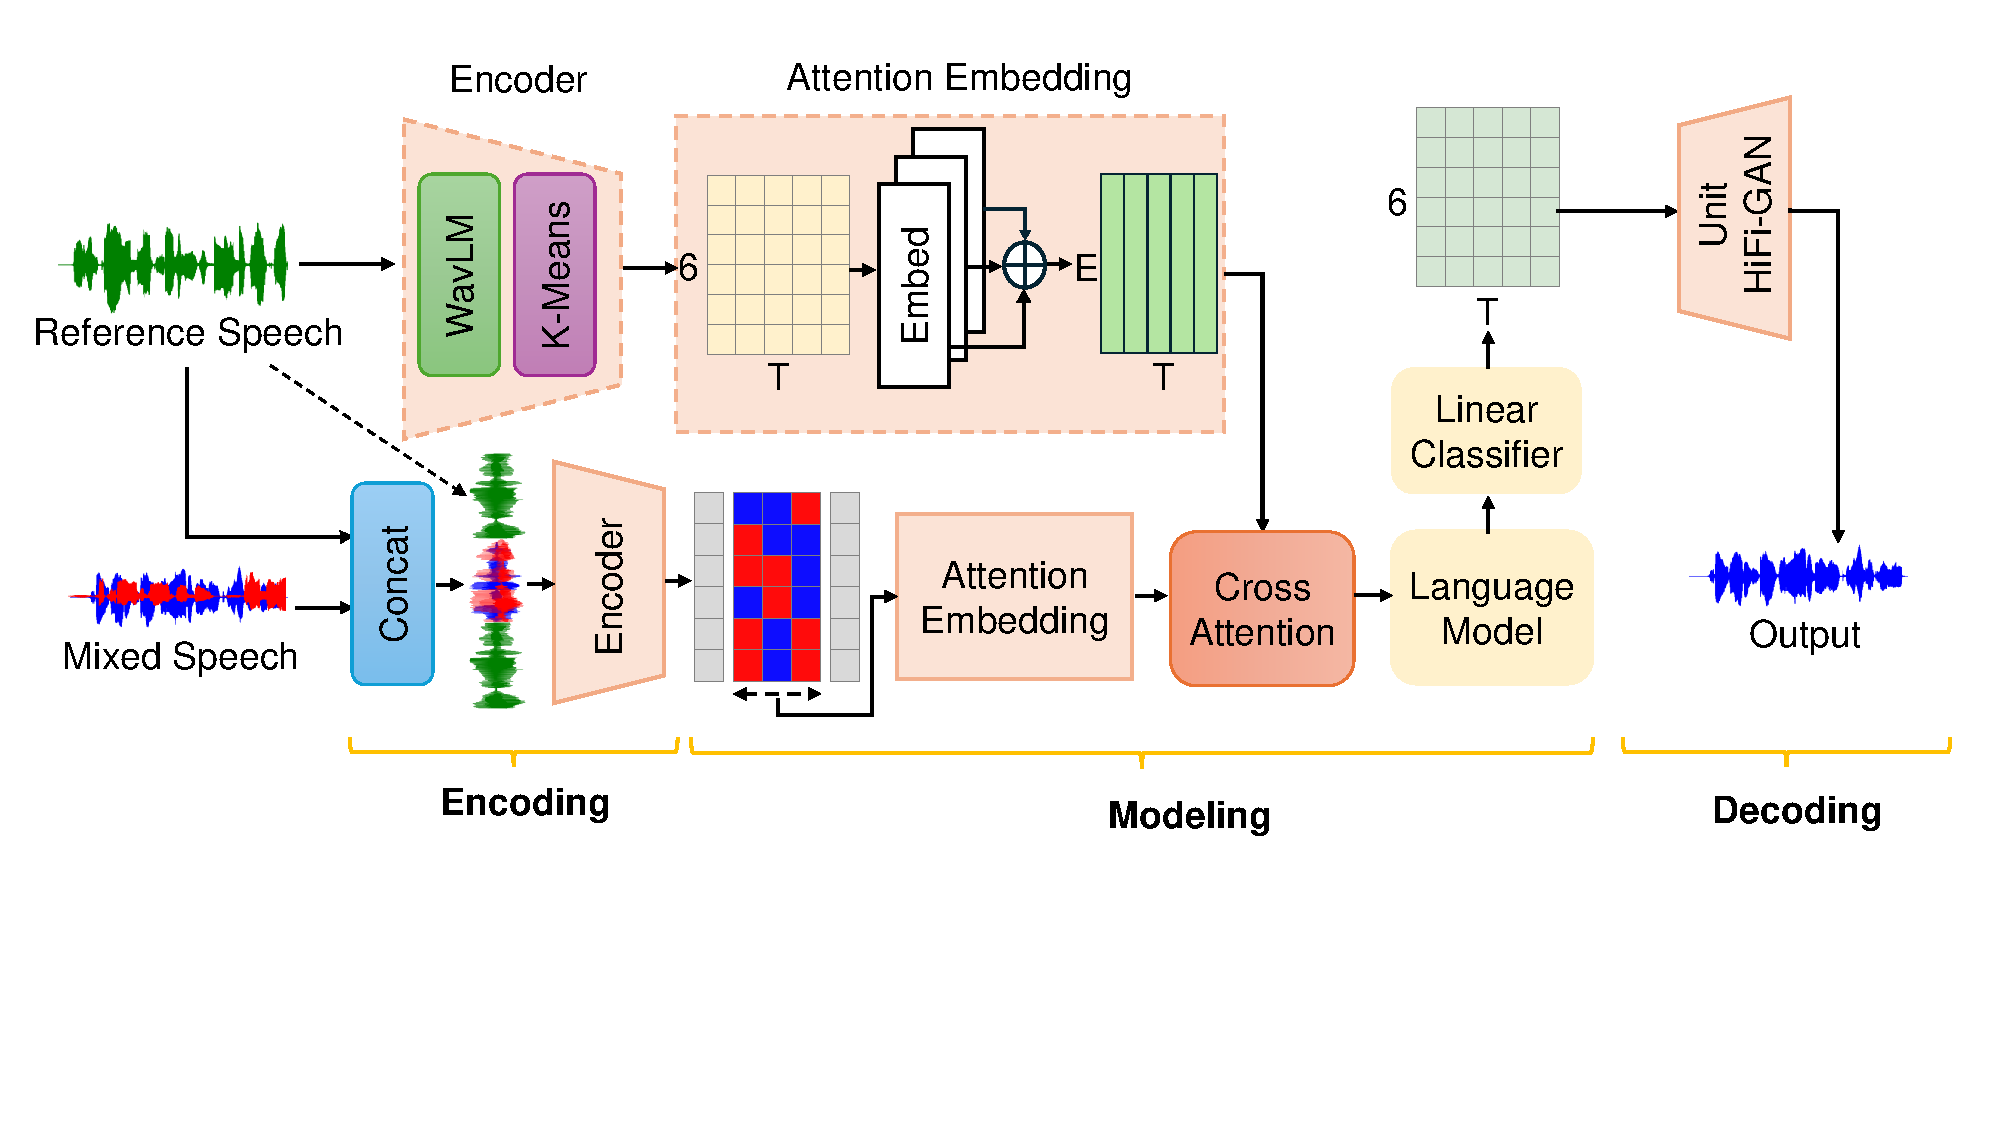
\includegraphics[width=\textwidth]{assets/model.pdf}
\caption{Overview of TSELM.}
\label{model}
\end{figure*}

\section{Method}

\subsection{Encoding}
We use pretrained SSL model WavLM Large \cite{wavlm} to 
encode the speech into continuous representations. We use the output from 6 hidden 
layers 1, 3, 7, 12, 18, 23. Given a speech signal \(s \in R^{T'} \), the output 
of WavLM will be a tensor \(\bm{r}\) of shape \(n \times T \times E\) where 
\(n\) specifies the number 
of output layers (6 in this case), and  \(T\) is the time 
dimension and \(E\) stands for the 
embedding dimension, specifically 1024 in WavLM Large. The Kmeans tokenizer uses \(n\) numbers of  Kmeans model 
separately on each output layer. Each model uses the same clustering number denoted by \(K\).
After tokenization, the continuous embedding \(\bm{r}\) will be transformed to a tensor \(\bm{d}\) of shape \(n \times T\) where each value \(\bm{d}_{(n_i,t)} \in (0, K-1), n_i \in (0,n), t \in 
(0, T)\). We choose \(K\) to be 1000 in our experiments. For reference speech and mixed speech, we 
use the same Kmeans model and the same layer output of WavLM. 

The encoding strategy on the mixed speech plays a pivotal role in the model performance. 
We follow the 
aforementioned procedure for 
reference speech to get tensor \(\bm{d_r}\) of shape \(n \times T_r\). But for the mixed 
speech, instead of directly following the procedure, we first concatenate it with 
the reference speech to get \(s' = [s_r, s_m, s_r] \in R^{()}\)

\subsection{Units}
\begin{itemize}
\item Use either SI (MKS) or CGS as primary units. (SI units are encouraged.) English units may be used as secondary units (in parentheses). An exception would be the use of English units as identifiers in trade, such as ``3.5-inch disk drive''.
\item Avoid combining SI and CGS units, such as current in amperes and magnetic field in oersteds. This often leads to confusion because equations do not balance dimensionally. If you must use mixed units, clearly state the units for each quantity that you use in an equation.
\item Do not mix complete spellings and abbreviations of units: ``Wb/m\textsuperscript{2}'' or ``webers per square meter'', not ``webers/m\textsuperscript{2}''. Spell out units when they appear in text: ``. . . a few henries'', not ``. . . a few H''.
\item Use a zero before decimal points: ``0.25'', not ``.25''. Use ``cm\textsuperscript{3}'', not ``cc''.)
\end{itemize}

\subsection{Equations}
Number equations consecutively. To make your 
equations more compact, you may use the solidus (~/~), the exp function, or 
appropriate exponents. Italicize Roman symbols for quantities and variables, 
but not Greek symbols. Use a long dash rather than a hyphen for a minus 
sign. Punctuate equations with commas or periods when they are part of a 
sentence, as in:
\begin{equation}
a+b=\gamma\label{eq}
\end{equation}

Be sure that the 
symbols in your equation have been defined before or immediately following 
the equation. Use ``\eqref{eq}'', not ``Eq.~\eqref{eq}'' or ``equation \eqref{eq}'', except at 
the beginning of a sentence: ``Equation \eqref{eq} is . . .''

\subsection{\LaTeX-Specific Advice}

Please use ``soft'' (e.g., \verb|\eqref{Eq}|) cross references instead
of ``hard'' references (e.g., \verb|(1)|). That will make it possible
to combine sections, add equations, or change the order of figures or
citations without having to go through the file line by line.

Please don't use the \verb|{eqnarray}| equation environment. Use
\verb|{align}| or \verb|{IEEEeqnarray}| instead. The \verb|{eqnarray}|
environment leaves unsightly spaces around relation symbols.

Please note that the \verb|{subequations}| environment in {\LaTeX}
will increment the main equation counter even when there are no
equation numbers displayed. If you forget that, you might write an
article in which the equation numbers skip from (17) to (20), causing
the copy editors to wonder if you've discovered a new method of
counting.

{\BibTeX} does not work by magic. It doesn't get the bibliographic
data from thin air but from .bib files. If you use {\BibTeX} to produce a
bibliography you must send the .bib files. 

{\LaTeX} can't read your mind. If you assign the same label to a
subsubsection and a table, you might find that Table I has been cross
referenced as Table IV-B3. 

{\LaTeX} does not have precognitive abilities. If you put a
\verb|\label| command before the command that updates the counter it's
supposed to be using, the label will pick up the last counter to be
cross referenced instead. In particular, a \verb|\label| command
should not go before the caption of a figure or a table.

Do not use \verb|\nonumber| inside the \verb|{array}| environment. It
will not stop equation numbers inside \verb|{array}| (there won't be
any anyway) and it might stop a wanted equation number in the
surrounding equation.

\subsection{Some Common Mistakes}\label{SCM}
\begin{itemize}
\item The word ``data'' is plural, not singular.
\item The subscript for the permeability of vacuum $\mu_{0}$, and other common scientific constants, is zero with subscript formatting, not a lowercase letter ``o''.
\item In American English, commas, semicolons, periods, question and exclamation marks are located within quotation marks only when a complete thought or name is cited, such as a title or full quotation. When quotation marks are used, instead of a bold or italic typeface, to highlight a word or phrase, punctuation should appear outside of the quotation marks. A parenthetical phrase or statement at the end of a sentence is punctuated outside of the closing parenthesis (like this). (A parenthetical sentence is punctuated within the parentheses.)
\item A graph within a graph is an ``inset'', not an ``insert''. The word alternatively is preferred to the word ``alternately'' (unless you really mean something that alternates).
\item Do not use the word ``essentially'' to mean ``approximately'' or ``effectively''.
\item In your paper title, if the words ``that uses'' can accurately replace the word ``using'', capitalize the ``u''; if not, keep using lower-cased.
\item Be aware of the different meanings of the homophones ``affect'' and ``effect'', ``complement'' and ``compliment'', ``discreet'' and ``discrete'', ``principal'' and ``principle''.
\item Do not confuse ``imply'' and ``infer''.
\item The prefix ``non'' is not a word; it should be joined to the word it modifies, usually without a hyphen.
\item There is no period after the ``et'' in the Latin abbreviation ``et al.''.
\item The abbreviation ``i.e.'' means ``that is'', and the abbreviation ``e.g.'' means ``for example''.
\end{itemize}
An excellent style manual for science writers is \cite{b7}.

\subsection{Authors and Affiliations}\label{AAA}
\textbf{The class file is designed for, but not limited to, six authors.} A 
minimum of one author is required for all conference articles. Author names 
should be listed starting from left to right and then moving down to the 
next line. This is the author sequence that will be used in future citations 
and by indexing services. Names should not be listed in columns nor group by 
affiliation. Please keep your affiliations as succinct as possible (for 
example, do not differentiate among departments of the same organization).

\subsection{Identify the Headings}\label{ITH}
Headings, or heads, are organizational devices that guide the reader through 
your paper. There are two types: component heads and text heads.

Component heads identify the different components of your paper and are not 
topically subordinate to each other. Examples include Acknowledgments and 
References and, for these, the correct style to use is ``Heading 5''. Use 
``figure caption'' for your Figure captions, and ``table head'' for your 
table title. Run-in heads, such as ``Abstract'', will require you to apply a 
style (in this case, italic) in addition to the style provided by the drop 
down menu to differentiate the head from the text.

Text heads organize the topics on a relational, hierarchical basis. For 
example, the paper title is the primary text head because all subsequent 
material relates and elaborates on this one topic. If there are two or more 
sub-topics, the next level head (uppercase Roman numerals) should be used 
and, conversely, if there are not at least two sub-topics, then no subheads 
should be introduced.

\subsection{Figures and Tables}\label{FAT}
\paragraph{Positioning Figures and Tables} Place figures and tables at the top and 
bottom of columns. Avoid placing them in the middle of columns. Large 
figures and tables may span across both columns. Figure captions should be 
below the figures; table heads should appear above the tables. Insert 
figures and tables after they are cited in the text. Use the abbreviation 
``Fig.~\ref{fig}'', even at the beginning of a sentence.

\begin{table}[htbp]
\caption{Table Type Styles}
\begin{center}
\begin{tabular}{|c|c|c|c|}
\hline
\textbf{Table}&\multicolumn{3}{|c|}{\textbf{Table Column Head}} \\
\cline{2-4} 
\textbf{Head} & \textbf{\textit{Table column subhead}}& \textbf{\textit{Subhead}}& \textbf{\textit{Subhead}} \\
\hline
copy& More table copy$^{\mathrm{a}}$& &  \\
\hline
\multicolumn{4}{l}{$^{\mathrm{a}}$Sample of a Table footnote.}
\end{tabular}
\label{tab1}
\end{center}
\end{table}

\begin{figure}[htbp]
\centerline{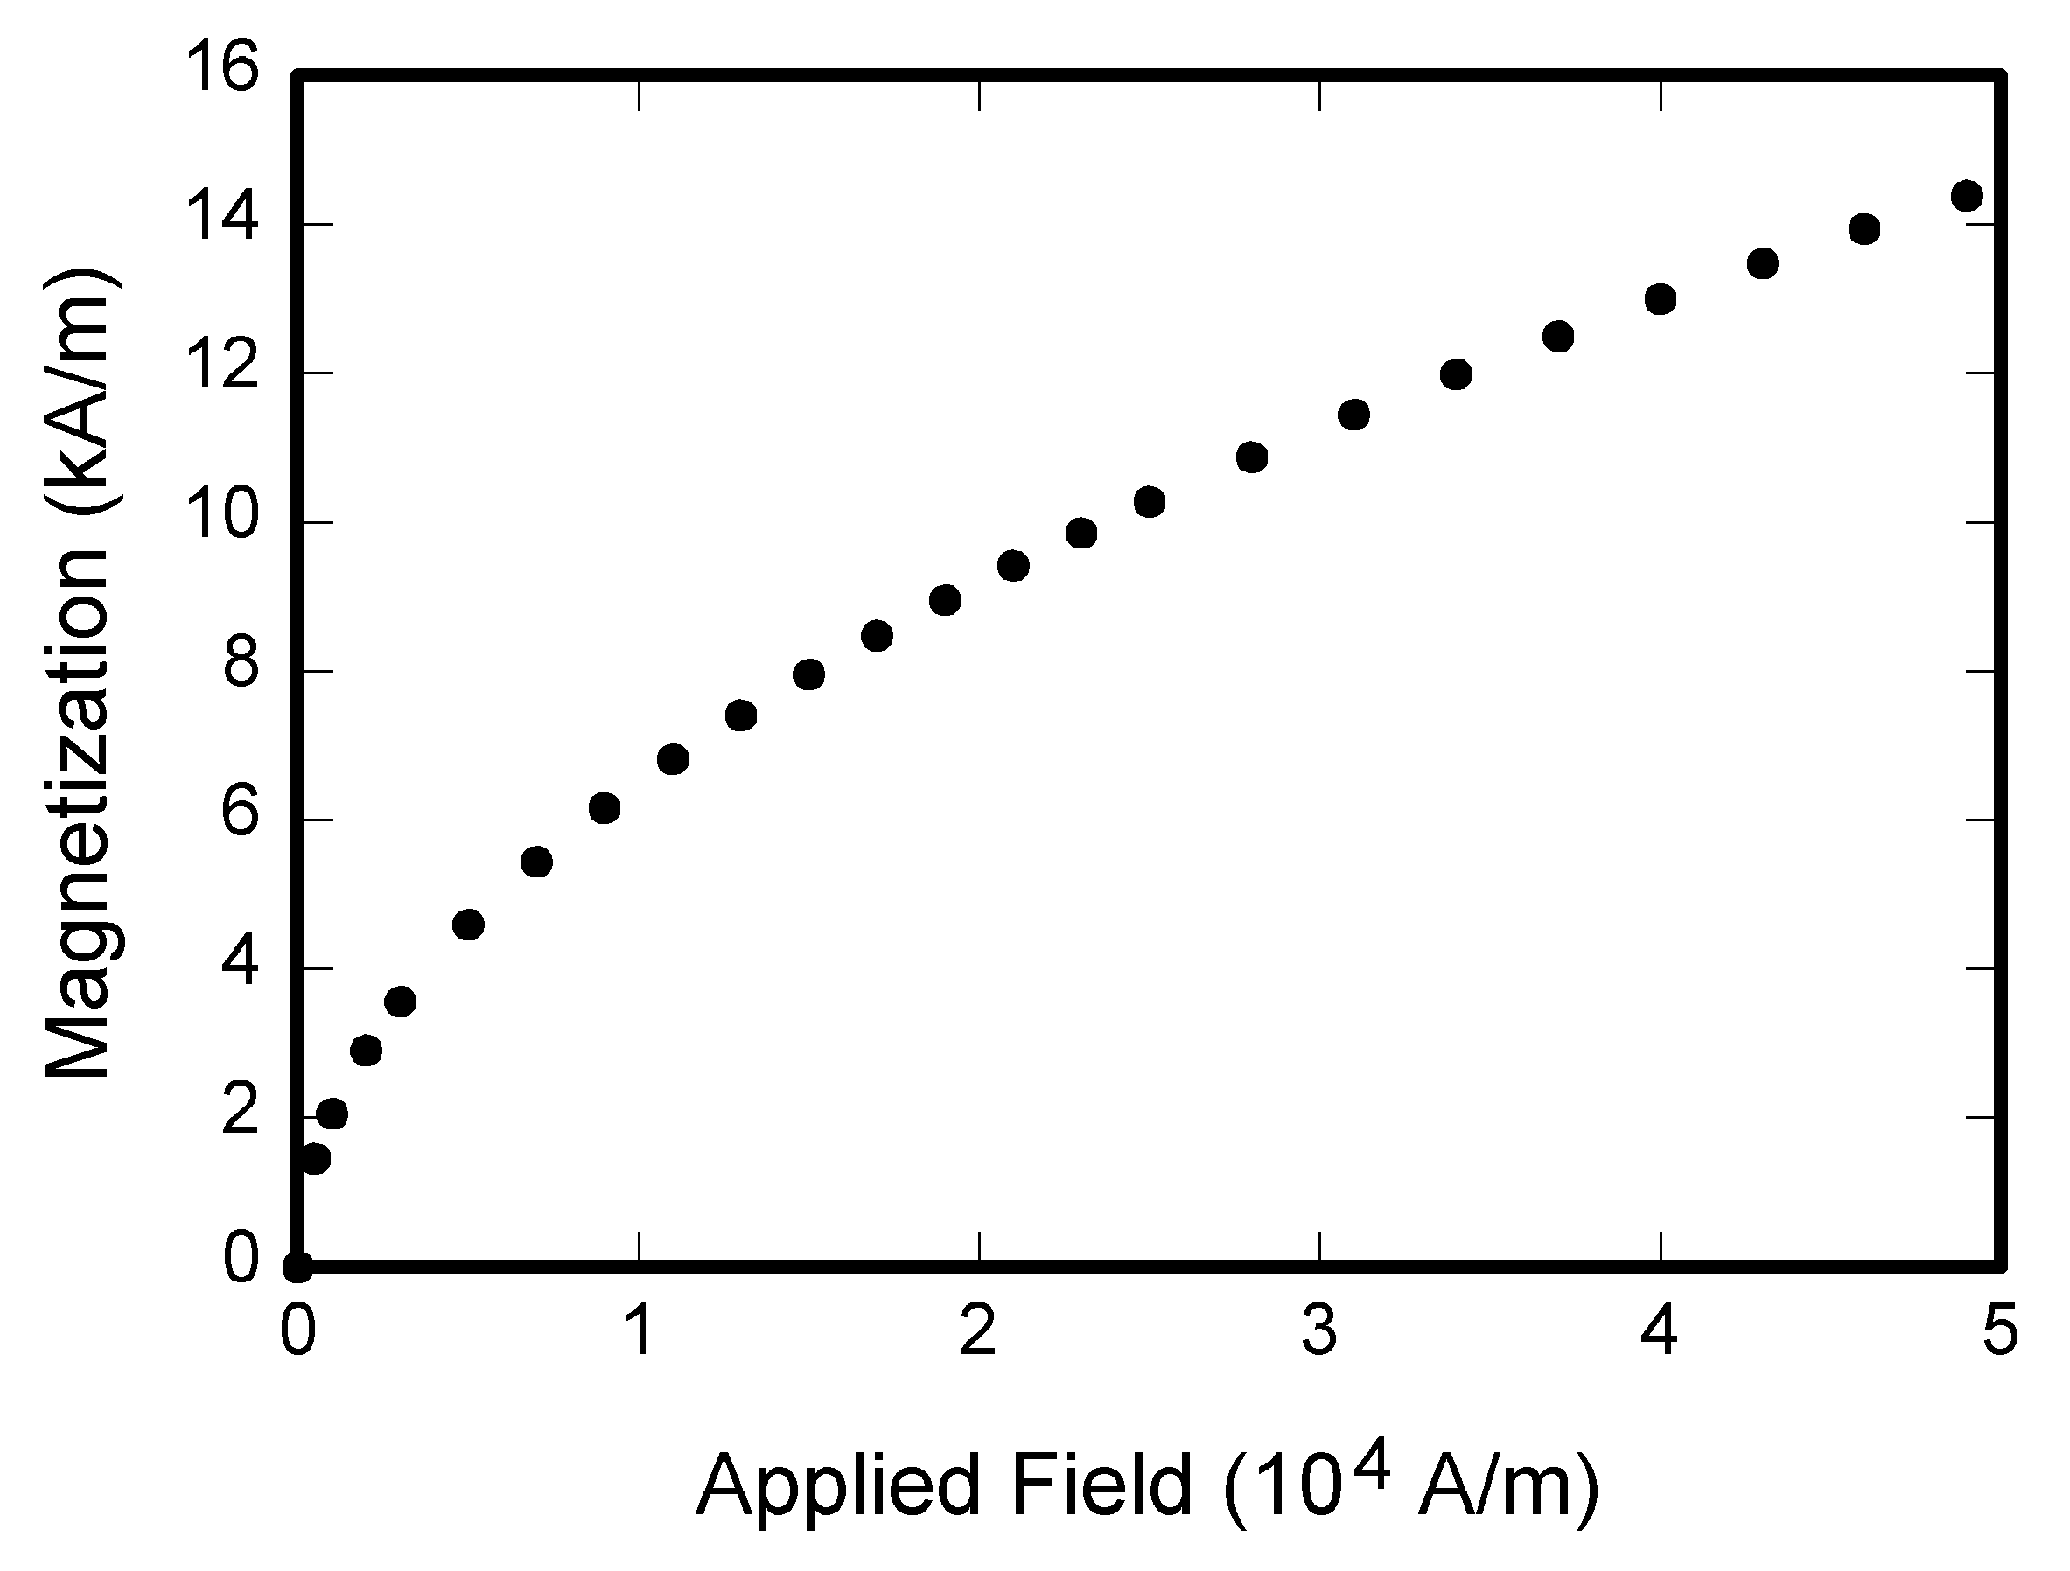
\includegraphics{fig1.png}}
\caption{Example of a figure caption.}
\label{fig}
\end{figure}

Figure Labels: Use 8 point Times New Roman for Figure labels. Use words 
rather than symbols or abbreviations when writing Figure axis labels to 
avoid confusing the reader. As an example, write the quantity 
``Magnetization'', or ``Magnetization, M'', not just ``M''. If including 
units in the label, present them within parentheses. Do not label axes only 
with units. In the example, write ``Magnetization (A/m)'' or ``Magnetization 
\{A[m(1)]\}'', not just ``A/m''. Do not label axes with a ratio of 
quantities and units. For example, write ``Temperature (K)'', not 
``Temperature/K''.

\section*{Acknowledgment}

The preferred spelling of the word ``acknowledgment'' in America is without 
an ``e'' after the ``g''. Avoid the stilted expression ``one of us (R. B. 
G.) thanks $\ldots$''. Instead, try ``R. B. G. thanks$\ldots$''. Put sponsor 
acknowledgments in the unnumbered footnote on the first page.

\section*{References}

Please number citations consecutively within brackets \cite{b1}. The 
sentence punctuation follows the bracket \cite{b2}. Refer simply to the reference 
number, as in \cite{b3}---do not use ``Ref. \cite{b3}'' or ``reference \cite{b3}'' except at 
the beginning of a sentence: ``Reference \cite{b3} was the first $\ldots$''

Number footnotes separately in superscripts. Place the actual footnote at 
the bottom of the column in which it was cited. Do not put footnotes in the 
abstract or reference list. Use letters for table footnotes.

Unless there are six authors or more give all authors' names; do not use 
``et al.''. Papers that \cite{b8} have not been published, even if they have been 
submitted for publication, should be cited as ``unpublished'' \cite{b4}. Papers 
that have been accepted for publication should be cited as ``in press'' \cite{b5}. 
Capitalize only the \cite{b11}  first word \cite{b9} in a paper title, except for proper nouns and 
element symbols.

For papers published in translation journals, please give the English \cite{b10}
citation first, followed by the original foreign-language citation \cite{b6}.
\bibliographystyle{IEEEtran}
\bibliography{references}

\vspace{12pt}
\color{red}
IEEE conference templates contain guidance text for composing and formatting conference papers. Please ensure that all template text is removed from your conference paper prior to submission to the conference. Failure to remove the template text from your paper may result in your paper not being published.

\end{document}
